\documentclass[conference]{IEEEtran}
\usepackage{graphicx}
\usepackage[utf8x]{inputenc}
\usepackage{longtable}
\usepackage[T1]{fontenc}
\usepackage{amsmath}

\ifCLASSINFOpdf
\else
\fi
\hyphenation{op-tical net-works semi-conduc-tor}


\begin{document}

\title{SecureIt: home security has never been so easy\\
Anno Accademico 2011/2012}

\author{
\IEEEauthorblockN{Luca Bonato, Marco Ziccardi}
\IEEEauthorblockA{Corso di studi in Informatica\\
Facoltà di Scienze MM.FF.NN.\\
Università degli Studi di Padova\\
Email: \{lohathe,marco.ziccard\}@gmail.com}
}


\maketitle


\begin{abstract}
Nowadays different applications offer a mechanism to monitor your home environment in order to detect any intrusion. None of that solutions completely exploits phone functionalities to find intruders: accelerometer, camera or microphone are often mutually exclusive. Moreover none of these applications tracks phone's position after an intrusion has been identified. The proposed application aims to collect different solution for motion/presence detection and to track phone's position using any kind of connectivity.
\end{abstract}

\IEEEpeerreviewmaketitle

\section{\textbf{Introduction}}

The aim of the application development was not only the creation of a home security system but the discovery of phone capabilities too. In fact operations performed by the application are complex and really resource needful:
\begin{itemize}
	\item Accelerometer to detect orientation and shake
	\item Camera to detect motion processing frames
	\item Microphone to detect environmental sound level
	\item Wifi or 3G connectivity to upload images and audio
	\item GPS to get current location
	\item Bluetooth to upload location in absence of connectivity
	\item In app encryption in order to securely authenticate the user
\end{itemize}

To the mobile application is associated a back-end where the application itself uploads images and audio got at the instant of intrusion detection.\\

\section{\textbf{Intrusion detection}}
Intrusion detection is done in three complementary ways:
\begin{itemize}
	\item \textbf{Accelerometer}
	\item \textbf{Camera}
	\item \textbf{Microphone}
\end{itemize}

	\subsection{Accelerometer}
The accelerometer is used to detect motion of the phone itself. Different sensitivity can be set in order to detect different kinds of motions.\\
The accelerometer returns a \textit{triple} of three acceleration values on the three axes (\textit{X}, \textit{Y} and \textit{Z}). 

\begin{figure}[!ht]
\begin{center}
\makebox[\linewidth]{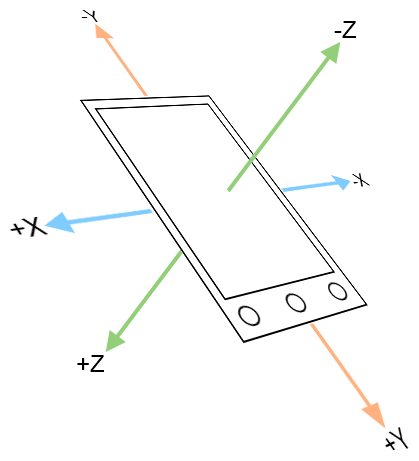
\includegraphics[scale=0.6]{resources/accelerometer.png}}
\caption{Values and signs of detected acceleration}
\end{center}
\end{figure}

Those values allow to detect every orientation taken by the phone except for phone rotations on the \textit{Z} axis when the phone is vertical (this is obvious according to the fact that in such a position the phone is not subject to acceleration variations on that axis).\\
Those acceleration values are used to move a 3D animation made in OpenGL ES (running on the GPU) that simply uses them to show phone's orientation, see figure \ref{img:opengl}.

\begin{figure}[!ht]
\begin{center}
\makebox[\linewidth]{
\includegraphics[scale=0.3]{resources/opengl.png}}
\caption{OpenGL ES 3D animation to show phone orientation}
\label{img:opengl}
\end{center}
\end{figure}


Acceleration triple is also used to detect any variation in the phone acceleration. Accelaration variation gives an idea of intensity of phone's \textit{shake} and it is computed as in equation \ref{eq:accel_variation}.\\

\begin{equation}
variation = \frac{(\Delta accelX)+(\Delta accelY)+(\Delta accelZ)}{\Delta t}
\label{eq:accel_variation}
\end{equation}
\vspace{.5cm}\\
Three levels of sensitivity are defined:
\begin{itemize}
	\item \texttt{LOW}: \texttt{SHAKE\_THRESHOLD = 5000}
	\item \texttt{MEDUM}:  \texttt{SHAKE\_THRESHOLD = 4000}
	\item \texttt{HIGH}:  \texttt{SHAKE\_THRESHOLD = 3000}
\end{itemize}

If $variation>SHAKE\_THRESHOLD$ the application starts to send alerts according to the specified options.

\subsection{\textbf{Camera}}
The camera is used to detect motion in the surrounding environment. The frames captured by the camera are processed to detect if any variation ha occurred since last captured frame.\\
A callback is activated at every captured frame, processing each captured frame would be too expensive for the phone in terms of CPU usage and battery consumption so the processing is reduced at one frame per second.\\
\subsubsection{\textbf{Motion detection}}
As said motion detection on the frame matrix is very expensive so the frames are scaled as soon as capture to a size of \texttt{640x480}. In order to detect any variation between two frames only the grayscale image is needed.\\
A movement is considered to be a difference in number of pixels between two grayscale frames bigger than a certain threshold.\\
In that case too we have three types of sensitivity, the sensitivity type defines not only the threshold in the number of different pixels (\texttt{NUMBER\_THRESHOLD}) but the threshold needed to consider different two pixels (\texttt{VALUE_THRESHOLD}):

\begin{itemize}
	\item \texttt{LOW}: \texttt{VALUE\_THRESHOLD = 60, NUMBER\_THRESHOLD = 20000}
	\item \texttt{MEDUM}: \texttt{VALUE\_THRESHOLD = 50, NUMBER\_THRESHOLD = 10000}
	\item \texttt{HIGH}: \texttt{VALUE\_THRESHOLD = 40, NUMBER\_THRESHOLD = 9000}
\end{itemize}

Rispetto ad un algoritmo globale un algoritmo locale nel caso in cui Pv, Pd e Po siano tutti negativi può iniziare un nuovo allineamento.\\
Il punteggio di un allineamento viene calcolato in maniera diversa nel caso in cui si stia lavorando su sequenze di aminoacidi o di nucleotidi:
\begin{itemize}
	\item \textbf{Aminoacidi}: il punteggio di allineamento è dato dalla somma di tutti i punteggi di appaiamento estratti da una \textit{scoring matrix} (sia essa PAM o BLOSUM) meno le penalità per i \textit{gap}. Le penalità per i \textit{gap} sono date da due componenti: la penalità di apertura di un \textit{gap} e la penalità conseguente all'allungamento di un residio (aminoacido) del \textit{gap}
	\item \textbf{Nucleotidi}: il punteggio è calcolato come sopra tranne per il fatto che la matrice di sostituzione è semplificata: +1 per un \textit{match}, -1 per un \textit{mismatch}
\end{itemize}
Le penalità di \textit{gap} sono variabili e dipendono dal contesto di utilizzo.

	\subsection{FASTA}

	Gli algoritmi di programmazione dinamica hanno risolto il problema dell'allineamento di due sequenze ma sono inutilizzabili (troppo lenti) per allineare una sequenza \textit{query} su tutte le sequenze \textit{subject} di una banca dati.\\


FASTA (Lipman e Pearson, 1985) è la prima soluzione euristica al problema dell'allineamento utilizzabile su una banca dati.\\
FASTA si basa su una strategia di indicizzazione di parole di \texttt{ktup} residui (nucleotidi o aminoacidi) dette \textit{k-mers}.
Tipicamente \texttt{ktup} = 6 per gli allineamenti di sequenze di nucleotidi e \texttt{ktup} = 2 per sequenze di aminoacidi.\\
FASTA scorre la \textit{query} e memorizza in un indice per ciascuna parola le posizioni in cui essa compare (costo lineare nella lunghezza della \textit{query}). Successivamente scorre ciascuna sequenza \textit{subject k-mer} per \textit{k-mer}, quando uno di questi compare nell'indice l'algoritmo memorizza la diagonale. Vengono poi calcolati i punteggi degli allineamenti di \textit{k-mer} tramite una matrice di sostituzione (PAM o BLOSUM a tolleranza variabile dipendentemente dal contesto), questo calcolo permette di escludere quelle sequenze \textit{subject} che non superano una certa soglia di similarità.\\
FASTA procede ad estendere ciascuno di questi allineamenti applicando opportune penalità per i \textit{gap} e anche in questo caso scarta le estensioni che non rientrano in una certa soglia di punteggio.\\
In ultima istanza viene eseguito Smith e Waterman modificato per considerare solo porzioni ristrette adiacenti alle estensioni appena calcolate ($\pm$ 20 aminoacidi).\\

FASTA per mezzo dell'indicizzazione delle parole identifica i \textit{match} possibili prima di effettuare una ricerca di allineamento più onerosa tramite Smith e Waterman.

	\subsection{BLAST}
BLAST (Altshul et al., 1990) rappresenta ad oggi l'algoritmo più usato per l'allineamento generale di proteine e DNA.\\
Risulta essere particolarmente efficiente negli allineamenti proteici poichè, invece di creare un indice basato sul \textit{matching} esatto delle parole (come FASTA), crea un indice basato sulla similarità calcolata per mezzo di una matrice di sostituzione (PAM o BLOSUM).\\
La lunghezza delle parole è definita da un parametro \texttt{W}, tipicamente nel caso di allineamento proteici \texttt{W}=3.\\
Dopo aver creato l'indice di similarità per la stringa \textit{query} l'algoritmo ricerca i \textit{W-mers} in tutte le sequenze \textit{subject} della base dati. Ogni corrispondenza può potenzialmente essere parte di un allineamento più lungo, si procede quindi all'estensione di tali corrispondenze in entrambe le direzioni ottendendo segmenti di allineamento locale non ulteriormente estendibili detti HSP (\textit{High-Scoring Segment Pair}). Un ulteriore parametro \texttt{X} determina quanto punteggio negativo può accumularsi nel tentativo di estendere una corrispondenza.\\


Tutti gli HSP che superano una certa soglia \texttt{S} sono ritenuti significativi.\\

Esistono diverse versioni di blast che realizzano compiti specifici:
\begin{itemize}
	\item \textbf{blastp}: ricerca gli allineamenti di una sequenza di aminoacidi su una banca dati di sequenze di aminoacidi
	\item \textbf{blastn}: ricerca gli allineamenti di una sequenza di nucleotidi su una banca dati di sequenze di nucleotidi
	\item \textbf{blastx}: ricerca allineamenti in una banca dati di sequenze proteiche a partire da una sequenza \textit{query} di nucleotidi dopo aver tradotto la \textit{query} in una sequenza di aminoacidi secondo tutte le 6 possibili fasi di lettura (\textit{6-frame translations})
	\item \textbf{tblastn}: ricerca gli allineamenti di una sequenza proteica su una banca dati di sequenze di nucleotidi calcolando per ciascuna sequenza \textit{subject} della banca dati tutte le possibili sequenze di aminoacidi (\textit{6-frame translations})
	\item \textbf{tblastx}: ricerca gli allineamenti di tutte le possibili traduzioni in sequenza di aminoacidi di una sequenza di nucleotidi con tutte le traduzioni in aminoacidi delle sequenze di una banca dati di nucleotidi. Rappresenta la versione più lenta dell'algoritmo BLAST, confronta sequenze aminoacidiche al posto di nucleotidi per offrire maggior tolleranza (effettua 36 confronti per ogni coppia di sequenze utilizzando matrici di sostituzione) e identificare relazioni di omologia tra sequenze nucleotidiche distanti
\end{itemize}

	\subsection{Burrows-Wheeler Transformation (BWT)}\label{sec:Burrows-Wheeler Transformation (BWT)}

\begin{table}[!ht]
\begin{center}
\begin{tabular}{|c|c|c|}
\textbf{Permutations} & \textbf{Sorted permutations} & \textbf{Last column}\\
\hline{}
&&\\
googol\$ & \$googol & \textbf{l} \\
&&\\
oogol\$g & gol\$goo & \textbf{o} \\
&&\\
ogol\$go & googol\$ & \textbf{\$} \\
&&\\
gol\$goo & l\$googo & \textbf{o} \\
&&\\
ol\$goog & ogol\$go & \textbf{o} \\
&&\\
l\$googo & ol\$goog & \textbf{g} \\
&&\\
\$googol & oogol\$g & \textbf{g} \\

\end{tabular}
\end{center}
\caption{BWT eseguita sulla stringa gogol (\$ indica la fine della stringa)}
\end{table}

Con l'avvento dei sequenziatori di nuova generazione il numero di \textit{reads} prodotte è aumentato notevolmente e consistentemente anche la quantità di genoma da allineare. Occorrevano metodi sempre più ottimizzati per la realizzazione dell'allineamento.\\
BWT (Burrows et al., 1994) è un algoritmo utilizzato nella compressione dei dati, sfruttato nel campo della bioinformatica per la creazione di indici di piccole dimensioni e di rapida consultazione.\\

BWT non cambia i valori dei caratteri che compaiono in una stringa ma semplicemente attua delle permutazioni tali che se la stringa in input conteneva caratteri ripetuti nella stringa trasformata questi appariranno di fila, rendendo così più facile la compressione.\\
La trasformazione viene banalmente fatta ordinando lessicograficamente tutte le permutazioni della stringa in input e prendendo l'ultima colonna.

\section{\textbf{Allineamento di reads corte}}

	\subsection{MAQ}
MAQ (Li et al., 2008), \textit{Mapping and Assembly with Qualities}, è un programma di allineamento che opera su \textit{reads} di piccole dimensioni prodotte da sequenziatori di nuova generazione, in particolare è progettato per lavorare con Illumina ma è in grado di lavorare anche con \textit{reads} prodotte da SOLiD (e quindi in \textit{color-space}).\\

MAQ differiva dalla maggior parte dei prodotti esistenti. In primo luogo calcola una misura di qualità per ciascun allineamento, misurante la probabibilità dell'allineamento di essere sbagliato (questo approccio aiuta notevolmente l'identificazione delle variazioni). In secondo luogo mappa ogni \textit{read} che abbia un \textit{match}, distribuendo casualmente le \textit{reads} ripetute in una delle alternative a parità di bontà, questo accorgimento solleva dall'ambiguità di definire il concetto di unica occorrenza di una \textit{read}. Inoltre MAQ allinea \textit{mate-pair reads} in una \textit{sliding window}, andando ad esaminare le posizioni accoppiate con poco costo computazionale e permettendo di allineare correttamente anche \textit{reads} ripetute se le loro \textit{mate reads} si trovano in regioni uniche.\\

Alcuni punti chiave dell'algoritmo MAQ sono:
	\begin{itemize}
		\item \textbf{Indicizzazione delle reads e scorrimento del genoma di riferimento}: le \textit{reads} sono indicizzate per mezzo di \textit{seeds} di 28 basi, si scorre il genoma di riferimento alla ricerca di \textit{seeds hit} con al più due \textit{mismatch}
		\item \textbf{Assegnazione di punteggi agli hit e mappatura casuale}: Ad un \textit{hit} viene assegnato un punteggio di $2^{24}*q+h$, dove \texttt{q} è la somma delle qualità delle basi che non si allineano correttamente e \texttt{h} è un intero in 24 bit derivante dall'\textit{hash} delle coordinate dell'\textit{hit} e dell'identificatore della \textit{read}. Come risultato MAQ mappa casualmente una \textit{read} se ci sono \textit{hit} ugualmente buone a causa di ripetizioni nel genoma
		\item \textbf{Qualità di allineamento}: La qualità di allineamento è la probabilità che l'allineamento di una \textit{read} sia sbagliato. Dato un genoma di riferimento \texttt{x} lungo \texttt{L} e una \textit{read} \texttt{z} lunga \texttt{l} la probabilità che \texttt{z} sia mappata in \texttt{u} è:
\begin{center}
$
p_s(u|x,z) = \frac{p(z|x,u)}{\sum_{v=1}^{L-l+1}p(z|x,v)}
$
\end{center}
Dove \texttt{p(z|x,u)} equivale al prodotto delle probabilità di errori delle basi che non si allineano. La qualità di un allineamento è:
\begin{center}
$
Q_s(u|x,z) = -10 log_{10}\left[1-p_s(u|x,z)\right]
$
\end{center}
		\item \textbf{Indels corti}: per le coppie di \textit{reads} tali che solo una viene allineata è utilizzato Smith e Waterman con \textit{gaps} per la \textit{read} associata in una regione ristretta determinata a seconda della dimensione dell'inserto, come in figura \ref{img:MAQ1}

		\item \textbf{Identificazione consensus}: forniti dei dati \texttt{D} di allineamento su una posizione si calcola $P(D|<b1,b1>)$, $P(D|<b2,b2>)$ e  $P(D|<b1,b2>)$, assumento che il campione su cui si sta lavorando sia diploide. La conoscenza della probabilità a priori di un eterozigote $<b1,b2>$ permette di calcolare la probabilità di ciascun genotipo. Il consensus $\hat g$ è il genotipo che massimizza la probabilità a posteriori e la sua qualità è $-10 log_{10}\left[1-P(\hat g|D)\right]$\\
	\end{itemize}

MAQ utilizza per l'allineamento 6 ore di CPU e 800MB di memoria per 1 milione di coppie di \textit{reads} ed è facilmente parallelizzabile su \textit{clusters}. Genera file binari compressi sia per gli allineamenti (1 byte per ciascun nucleotide delle \textit{reads}) sia per il consensus (4 byte per ciascun nucleotide sul genoma di riferimento). Fornisce inoltre un visualizzatore dei risultati dell'allineamento detto \textit{maqview} che permette di identificare graficamente la posizione di una qualsiasi \textit{read} sul genoma.\\

Le prestazioni di MAQ sono riassunte in figura \ref{img:MAQ2} e sono state estratte dai dati di allineamento di 100 millioni di coppie di \textit{reads} da 35 basi (estratte da un campione diploide con 0.1\% di sostituzioni e 0.01\% di \textit{indels} di una base) sul genoma umano.

	\subsection{Bowtie}
Bowtie (Langmead et al., 2009) usa un indice costruito tramite \textit{Burrows-Wheeler Transformation} e promette di avere una piccola occupazione di memoria (circa 1.3GB per l'intero genoma umano).\\

Bowtie effettua alcuni compromessi per fornire la sua velocità e il suo scarso utilizzo di memoria, esso infatti non garantisce la più alta qualità di \textit{mapping} delle \textit{reads} se non esiste alcun \textit{match} esatto. Inoltre può fallire nell'allineare alcune \textit{reads} quando configurato per eseguire alla massima velocità. Possiede diverse opzioni per bilanciare questo \textit{trade-off}.

	\subsection{BWA}
	BWA (Li e Durbin, 2009), \textit{Burrows-Wheeler Aligner}, può essere visto come una evoluzione di MAQ. Mentre MAQ utilizza un indice basato su \textit{hash} per cercare il genoma di riferimento BWA utilizza un indice costruito con BWT che permette ricerche più veloci del suo predecessore.\\

		\subsubsection{Prefix trie e string matching}
		Un \textit{prefix trie} per una stringa \texttt{X} è un albero in cui ogni arco è etichettato con un simbolo e la concatenazione delle etichette nel cammino da una foglia alla radice rappresenta un prefisso di \texttt{X}. Dato un \textit{prefix trie} cercare se una \textit{query} \texttt{W} è una sottostringa esatta di \texttt{X} equivale a cercare il nodo che rappresenta \texttt{W} e ciò può essere fatto in tempo \texttt{O(|W|)}. Per consentire \textit{mismatch} possiamo compiere un attraversamento esaustivo dell'albero e confrontare \texttt{W} con ogni possibile cammino.\\

		\subsubsection{BWT e suffix array}
		Supponiamo di aver calcolato la \textit{Burrows-Wheeler Transformation} e di averla memorizzata in \texttt{B}. Un \textit{suffix array} \texttt{S} di una stringa \texttt{X} lunga \texttt{n} è una permutazione degli indici \texttt{0 ... n-1} tale che \texttt{S[i]} è la posizione iniziale dell'i-esimo suffisso più piccolo.\\

La maggior parte degli algoritmi per la costruzione di un \textit{suffix array} richiedono \texttt{O(nlogn)} in memoria, risultando in $\tilde{12GB}$ per l'intero genoma umano, recentemente Hon et al. (2007) hanno presentato una nuova tecnica che permette di costruire l'albero dei suffissi per l'intero genoma umano in spazio (nei picchi) <1GB. Tale tecnica è adottata da BWA.\\

		\subsubsection{Intervalli nel suffix array}
		Se una stringa \texttt{W} è una sottostringa di \texttt{X}, la posizione di ogni occorrenza di \texttt{W} in \texttt{X} si troverà in un intervallo nel \textit{suffix array} dal momento che tutti i suffissi contenenti \texttt{W} sono ordinati insieme. Definiamo quindi:\\
\begin{center}
$\bar{R}$(W) = max\{k : W è prefisso di X$_{S(k)}$\}\\
$\underline{R}$(W) = min\{k : W è prefisso di X$_{S(k)}$\}\\ 
\end{center}

		\subsubsection{Matching esatto}
		Sia \texttt{C(a)} il numero di simboli in \texttt{X[0,n−2]} che sono lessicograficamente minori di un \texttt{a} appartenente all'alfabeto e \texttt{O(a,i)} il numero di occorrenze di \texttt{a} in \texttt{B[0,i]}. Ferragina e Manzini (2000) provarono che, se \texttt{W} è una sottostringa di \texttt{X}, allora:
\begin{center}
$\bar{R}$(aW) = C(a)+O(a,$\underline{R}$(W))\\
$\underline{R}$(aW) = C(a)+O(a,$\bar{R}$(W)−1)+1
\end{center}
Questo risultato permette di controllare se \texttt{W} è una sottostringa di \texttt{X} e contare le occorenze di \texttt{W} in tempo \texttt{O(|W|)} calcolando iterativamente \texttt{$\bar{R}$} e \texttt{\underline{R}} a partire dalla fine di \texttt{W}. Questa procedura è chiamata \textit{backward search}.\\

		\subsubsection{Matching non esatto}
		L'algoritmo data una stringa \texttt{W} cerca gli intervalli nel \textit{suffix array} di \texttt{X} delle sottostringhe che hanno un \textit{match} con \texttt{W} con non più di \texttt{z} differenze. Essenzialmente la ricerca di un \textit{match} non esatto usa \textit{backward search} per campionare sottostringhe distinte dal genoma. Questo processo è limitato dall'\textit{array} \texttt{D}, tale che \texttt{D[i]} è il limite inferiore al numero di differenze in \texttt{W[0,i]}. Meglio è stimato \texttt{D} più si restringe lo spazio di ricerca nel \textit{suffix trie} e quindi più è efficiente l'algoritmo. Un \textit{bound} semplice per \texttt{D} è \texttt{D[i]=0} per ogni \texttt{i} ma questo risulta in un algoritmo molto inefficiente.\\

		\subsubsection{Valutazione delle prestazioni}
		Nel valutare le prestazioni di BWA sono state utilizzate quelle di altri tre programmi: MAQ, SOAPv2 e Bowtie. MAQ indicizza le \textit{reads} tramite una \textit{hash table} mentre SOAPv2 e Bowtie sono altri due algoritmi che utilizzano BWT.
Sono stati condotti esperimenti sia con dati simulati sia con dati reali.\\

\begin{table}
\begin{center}
\begin{tabular}{|c|ccc|ccc|}
	& \multicolumn{3}{c|}{Single-end} & \multicolumn{3}{c|}{Paired-end} \\
Program & Time(s) & Conf(\%) & Err(\%) & Time(s) & Conf(\%) & Err(\%)\\
\hline{}
& & & & & & \\
Bowtie-32 & 1271 & 79.0 & 0.76 & 1391 & 85.7 & 0.57 \\
& & & & & & \\
BWA-32 & 823 & 80.6 & 0.30 & 1224 & 89.6 & 0.32 \\
& & & & & & \\
MAQ-32 & 19797 & 81.0 & 0.14 & 21589 & 87.2 & 0.07 \\
& & & & & & \\
SOAP2-32 & 256 & 78.6 & 1.16 & 1909 & 86.8 & 0.78 \\
& & & & & & \\
\hline{}
& & & & & & \\
Bowtie-70 & 1726 & 86.3 & 0.20 & 1580 & 90.7 & 0.43 \\
& & & & & & \\
BWA-70 & 1599 & 90.7 & 0.12 & 1619 & 96.2 & 0.11 \\
& & & & & & \\
MAQ-70 & 17928 & 91.0 & 0.13 & 19046 & 94.6 & 0.05 \\
& & & & & & \\
SOAP2-70 & 317 & 90.3 & 0.39 & 708 & 94.5 & 0.34 \\
& & & & & & \\
\hline{}
& & & & & & \\
Bowtie-125 & 1966 & 88.0 & 0.07 & 1701 & 91.0 & 0.37 \\
& & & & & & \\
BWA-125 & 3021 & 93.0 & 0.05 & 3059 & 97.6 & 0.04 \\
& & & & & & \\
MAQ-125 & 17506 & 92.7 & 0.08 & 19388 & 96.3 & 0.02 \\
& & & & & & \\
SOAP2-125 & 555 & 91.5 & 0.17 & 1187 & 90.8 & 0.14 \\
\end{tabular}

\end{center}
\caption{Prestazioni di BWA per l'allineamento di un milione di coppie di \textit{reads} di 32, 70 e 125 basi simulate da un genoma umano con frequenza di SNP (\textit{Single Nucleotide Polimorphism}) pari a 0.09\%, una frequenza di \textit{indels} pari a 0.01\% una frequenza uniforme di errori di sequenziamento di 2\%. Sono mostrati i tempi di esecuzione (calcolati su un \textit{core} del processore 2.5 GHz Xeon E5420I), la stima percentuale di \textit{reads} allineate correttamente e la percentuale di errore in tale stima}
\label{tab:BWA1}
\end{table}

\begin{itemize}
	\item \textbf{Dati simulati:} 
Sono state simulate \textit{reads} dal genoma umano con lo strumento \textit{wgsim} incluso nel pacchetto \textit{SAMtools} e successivamente sono stati eseguti i quattro programmi per allineare tali \textit{reads} sul genoma umano. La tabella \ref{tab:BWA1} mostra come BWA e MAQ raggiungano la stessa accuratezza nell'allineamento mentre BWA risulta essere più preciso sia di SOAPv2 che di Bowtie. Per quanto concerne la velocità SOAPv2 è decisamente il più veloce per l'allineamento \textit{single-end} ma viene recuperato nell'allineamento \textit{paired-end} nel quale BWA risulta essere migliore in due casi su tre (\textit{reads} di 32 e 125 basi).\\
Per quello che riguarda la memoria SOAPv2 usa 5.4GB. Sia Bowtie che BWA utilizzano 2.3GB per l'allineamento \textit{single-end} mentre circa 3GB per il \textit{paired-end}, più grande della memoria necessaria a MAQ che è di circa 1GB. Tuttavia l'utilizzo di memoria negli algoritmi basati su BWT non dipende dal numero di \textit{reads} da allineare mentre l'occupazione di MAQ è lineare in esso. Inoltre gli allineatori centrati su BWT supportano il \textit{multi-threading}.\\
	\item \textbf{Dati reali:}
	L'allineamento è stato fatto utilizzando 12.2 milioni di coppie di \textit{reads} di 51 basi prodotte dal sequenziatore Illumina. Le prestazioni misurate sono mostrate in tabella \ref{tab:BWA2}.

\begin{table}
\begin{center}
\begin{tabular}{c c c c}
Program & Time(h) & Conf(\%) & Paired(\%) \\
\hline{}
&&&\\
Bowtie & 5.2 & 84.4 & 96.3 \\
&&&\\
BWA & 4.0 & 88.9 & 98.8 \\
&&&\\
MAQ & 94.9 & 86.1 & 98.7 \\
&&&\\
SOAP2 & 3.4 & 88.3 & 97.5 \\
\end{tabular}
\end{center}
\caption{Sono mostrati i tempi di esecuzione (calcolati su un \textit{core} del processore 2.5 GHz Xeon E5420I), la stima percentuale di \textit{reads} allineate correttamente e la stima percentuale con le \textit{mate-pairs} mappate nel corretto orientamento da BWA}
\label{tab:BWA2}
\end{table}

\end{itemize}
		

	\subsection{mrFAST e mrsFAST}
	I programmi mr- e mrsFAST (Alkan et al., 2009; Hach et al., 2010) sono degni di nota dal momento che restituiscono tutti i possibili allineamenti di una \textit{read} su un genoma, non soltanto l'unico allineamento migliore. L'abilità di riportare tutte le possibili locazioni del genoma è molto utile per l'identificazione delle variazioni strutturali, infatti questi due algoritmi sono stati sviluppati proprio a questo scopo.\\

mr- e mrsFAST utilizzano un metodo \textit{seed-and-extend} per l'allineamento, creano indici di una \textit{hash table} per il genoma di riferimento, ciascuna \textit{read} viene suddivisa in \textit{first middle} e \textit{last k-mers} (di default \texttt{k}=12), ciascuno di questi \textit{k-mer} viene cercato nel \textit{hash} per fissare i \textit{seeds} di allineamento.

	\subsection{BFAST}
	BFAST (Homer et al., 2009) è un algoritmo per allineare \textit{reads} corte su un genoma di riferimento di grandi dimensioni.\\
	Realizza l'allineamento in due fasi:
	\begin{itemize}
		\item Crea indici multipli sul genoma di riferimento
		\item Identifica le CAL (\textit{Candidate Alignment Locations}) per ciascuna \textit{read}, successivamente queste CAL sono allineate localmente usando \textit{gap} per identificare il miglior \textit{match}. Questa tecnica si applica alle sequenze in \textit{base-space} (Illumina e 454) e in \textit{color-space} (SOLiD). L'allineamento usando \textit{gap} permette di identificare SNP (\textit{Single Nucleotide Polimorphism}), inserzioni e delezioni, oltre che errori nella sequenza in \textit{color-space}\\
	\end{itemize}

	BFAST utilizza un indice multiplo prestando bene attenzione a sfruttarlo il più possibile quando esso viene caricato in RAM.
	Ciascun indice è un \textit{suffix array} ottimizzato del genoma di riferimento che indicizza un \textit{seed}, una stringa di 0 e 1 che inizia e finisce con 1, che definisce le basi nella \textit{read} che si stanno considerando in un \textit{lookup}.\\
Chiamiamo \texttt{k} (\textit{key size}) il numero di 1 in un \textit{seed} mentre \texttt{w} (\textit{key width}) il numero di 0 e 1. Il numero di CAL identificate dall'algoritmo dipende da \texttt{k} e dalla complessità e quantità di ripetizioni presenti nel genoma di riferimento. Con \texttt{k} maggiori in media si ha un \textit{lookup} più probabilmente unico nell'indice ma si riduce anche il numero di \textit{lookup} totali, rendendo l'algoritmo meno sensibile.\\
Solitamente per il genoma umano viene preferito \texttt{k} = 18 per \textit{reads} corte ($\le$ 40 bp) e \texttt{k} = 22 per \textit{reads} più lunghe ($\ge$ 40 bp) per bilanciare sensibilità e unicità del \textit{lookup}. Scegliere \texttt{k} di minori dimensioni è utile per le \textit{reads} corte dal momento che così aumenta il numero di \textit{offsets} e la sensibilità migliora.\\
BFAST implementa un \textit{hash} verso l'indice che riduce il tempo di \textit{lookup} e consiste delle prime \texttt{j} basi (\texttt{j} è detta \textit{hash width}) degli indici di riferimento, con \texttt{j} $\le$ \texttt{k}. \textit{Hash width} è sempre più corta di \textit{key size}.\\

La RAM necessaria per caricare un intero indice è approssimativamente 17GB, che porta in pratica alla necessità di 24GB di RAM per prestazioni ottime, quantità elevata ma raggiungibile dai moderni computer. Inoltre BFAST è in grado di scomporre l'indice in $4^n$ componenti: in questo modo, nonostante la fase di \textit{lookup} richieda più tempo dal momento che essa andrà replicata su ogni indice parziale, BFAST per l'intero genoma riesce ad eseguire su computer con solo 4GB di RAM.\\

BFAST ammette allineamenti \textit{paired-end} o \textit{mate-pair}, realizzando allineamenti indipendenti per ciascun \textit{end} e annotando il collegamento tra \textit{pair-ends}.\\


Per mostrare le performance di BFAST esso è stato confrontato con altri software disponibili utilizzando \textit{reads} diverse per dimensione e tipo. A questo scopo sono stati utilizzati sia dati simulati che dati reali.\\

Nelle figure \ref{img:BFASTperf1}, \ref{img:BFASTperf2}, \ref{img:BFASTperf3} viene effettuata una valutazione degli algoritmi di allineamento su un insieme di 10,000 \textit{reads} simulate in \textit{base-space}.\\

\begin{table}
\begin{center}
\begin{tabular}{|c|c|c|c|c|}
& Illumina & Illumina & ABI SOLiD & ABI SOLiD \\
& 3.5M 55bp & 3.5M 55bp & 1M 50bp & 1M 50bp \\
& Time (s) & \% mapped & Time (s) & \% mapped \\
\hline{}
&&&&\\
BFAST & 47,474 & 69.6 & 42,856 & 72.5 \\
&&&&\\
BOWTIE & 857 & 55.7 & not supported & not supported \\
&&&&\\
BWA & 4,883 & 59.3 & 845 & 47.8 \\
&&&&\\
MAQ & 126,541 & 73.6 & 6,680 & 68.1 \\
&&&&\\
SHRiMP & 324,380 & 83.3 & 32,644 & 70.4 \\
&&&&\\
SOAP & 131,248 & 62.4 & 131,248 & 62.4 \\
&&&&\\
\end{tabular}
\end{center}
\caption{Risultati nei tempi di allineamento e nel numero di \textit{reads} allineate correttamente di vari algoritmi su due \textit{datasets} reali differenti in relazione a tempi e percentuali di BFAST}
\label{tab:BFASTperf4}

\end{table}

In tabella \ref{tab:BFASTperf4} i tempi di allineamento sono stati calcolati su due tipologie di \textit{reads}, prodotte in un caso da Illumina in \textit{base-space} e nel secondo caso da SOLiD in \textit{color-space}, è mostrata inoltre la percentuale di \textit{reads} allineate correttamente.

	\subsection{Novoalign}
	Novoalign è un prodotto proprietario di Novocraft (Novocraft, 2000) che utilizza una strategia di \textit{hashing} simile a MAQ (Li et al., 2008).\\

Novoalign è diventato piuttosto popolare nelle recenti pubblicazioni a causa della sua accuratezza, esso inoltre ammette fino a 8 \textit{mismatch} per \textit{read} nell'allineamento di una sola \textit{end}.

	\subsection{SHRiMP}

SHRiMP (Rumble et al., 2009) è un programma di allineamento specializzato nel mappare \textit{reads} in \textit{color-space} generate dal sequenziatore SOLiD. Dal momento che la conversione di sequenze da \textit{base-space} a \textit{color-space} è univoca è possibile utilizzarlo anche per quest'ultime.\\
SHRiMP utilizza tutti i recenti avanzamenti nell'allineamento di sequenze:
\begin{itemize}
	\item \textit{Q-gram filters} (Rasmussen et al., 2005): che consentono di cominciare l'allineamento con \textit{seeds} che abbiano più di un \textit{match}
	\item \textit{Spaced seeds} (Califano and Rigoutsos, 1993): che ammettono sezioni di \textit{mismatch} predeterminate nelle sequenze \textit{seed}s
	\item Hardware specializzato: implementazioni ed istruzioni particolari che permettono di velocizzare l'algoritmo standard Smith e Waterman\\
\end{itemize}
SHRiMP è stato ulteriormente migliorato nella sua versione successiva SHRiMP2 (David et al. 2010). Quest'ultima versione si distingue dalla precedente andando essa ad indicizzare non le \textit{reads} ma il genoma di riferimento. Tale modifica ha notevolmente migliorato le prestazioni permettendo l'aggiunta di una modalità per l'allineamento \textit{paired-end} e ha aperto la strada al \textit{multi-threading}.\\

L'indice del genoma di riferimento è caricato in RAM, per l'intero genoma umano arriva ad occupare 48GB. SHRiMP2 offre tuttavia degli strumenti per scomporre tale indice in componenti che rientrino in una certa quantità di RAM. L'\textit{overhead} prodotto da questa suddivisione può essere trascurato.\\

Diversi \textit{threads} sono usati per allineare le \textit{reads}. Utilizzando dei \textit{seeds} sono letti e cercati nell'indice tutti i possibili \textit{k-mer} della \textit{reads}. Tali posizioni dell'indice corrispondono a delle diagonali nella matrice di allineamento. Date queste diagonali è possibile costruire un insieme di CML (\textit{Candidate Mapping Locations}).\\

SHRiMP2 utilizza un meccanismo di \textit{caching} per velocizzare l'allineamento di \textit{reads} provenienti da sequenze ripetute: dopo ciascun all'ineamento viene calcolato un \textit{hash} della regione e salvato il punteggio, in caso di successive richieste per quella regione il punteggio non sarà ricalcolato.\\

L'unico programma che sia effettivamente confrontabile con SHRiMP2 è BFAST in quanto gli intenti di sviluppo sono praticamente gli stessi: preferire la correttezza alla velocità. Come BFAST, SHRiMP2 garantisce alta precisione anche per \textit{reads} molto polimorfe. Nei test SHRiMP2 raggiunge una precisione simile o addirittura maggiore a quella di BFAST per tutti i tipi di polimorfismo, eseguendo inoltre tra le 2 e le 5 volte più velocemente.

	\subsection{ABMapper}
	Gli allineatori di \textit{reads} corte generate dai moderni sequenziatori forniscono un'idea dell'allineamento ma non sono in grado di gestire adeguatamente \textit{reads} provenienti da sequenziamento di RNA che si trovino a cavallo di posizioni tra le quali è avvenuto \textit{splicing} o che appartengano a sequenze ripetute e che possono quindi essere mappate su più posizioni nel genoma.\\

ABMapper (Chan et al., 2010) vuole essere uno strumento in grado di analizzare \textit{reads} a cavallo di regioni che abbiano subito \textit{splicing} o appartenenti a regioni ripetute.\\

La sequenza genomica di riferimento è inizialmente inidicizzata in \textit{k-mers} secondo un \texttt{k} definito dall'utente. Dopo l'indicizzazione per ciascuna \textit{read} che si vuole allineare sono estratti due \textit{seeds} (chiamati \texttt{A} e \texttt{B}, dai quali deriva il nome del programma) di lunghezza \texttt{k} da ciascuna estremità della \textit{read} e sono estesi tramite allineamento uno verso l'altro, come in figura \ref{img:ABMapper}.\\


Due scenari possono manifestarsi durante l'estensione di un \textit{seed}:
\begin{itemize}
	\item \textit{Exonic alignment}: la \textit{read} non si trova a cavallo di due regioni che hanno subito \textit{splicing}, viene esteso soltanto un \textit{seed}
	\item \textit{Spliced alignment}: entrambi i \textit{seeds} sono estesi finchè non viene trovato un punto di terminazione. Un buon allineamento in questo caso prevede che i due \textit{seeds} siano estesi indipendentemente fino a che l'intera \textit{read} non è coperta. Se l'allungamento tollera errori però un \textit{seed} può essere esteso oltre il suo reale punto di terminazione. In questi casi l'algoritmo tollererà e correggerà le sovrapposizioni\\
\end{itemize}

ABMapper supporta diversi formati in input: semplici file di testo, FASTA e FASTQ. Inoltre ABMapper è in grado di estrarre \textit{reads} mappate su più di una posizione nel genoma o non mappate da file SAM/BAM prodotti da BWA per tentare un ulteriore allineamento.\\

La lunghezza \texttt{k} di un \textit{seed} determina la velocità di ricerca, la sensibilità e la precisione, più essa è corta più l'allineamento diventa accurato ma aumentano i tempi di esecuzione. ABMapper permette all'utente di definire tale dimensione coerentemente con la dimensione del campione (numero di \textit{reads} da allineare) e la potenza di calcolo a disposizione. La dimensione di default è 10.\\

ABMapper tollera dinamicamente l'errore ammettendo che alcune \textit{reads} siano ulteriormente estese oltre il loro limite eventualmente accettando un ulteriore errore che supera quello di \textit{cutoff}. Questa tecnica è molto utile nel caso di \textit{paired-end reads} che sono affette dal problema noto secondo il quale la seconda \textit{read} ha una qualità inferiore (errori maggiormente frequenti) rispetto alla prima.\\ Un'altra funzionalità importante è quella di ammettere sovrapposizioni tra frammenti di una \textit{read} che abbia subito \textit{splicing}, la regione sovrapposta può essere ulteriormente analizzata.\\

ABMapper è in grado di identificare probabili siti di \textit{splicing} utilizzando motivi canonici come \texttt{GT-AG}, \texttt{GC-AG} e \texttt{AT-AC} per riconoscere possibili giunzioni, specialmente nel caso in cui nell'estensione siano identificati due frammenti sovrapposti.\\

Elementi ripetuti nella sequenza possono essere filtrati secondo un numero di ripetizioni soglia specificato dall'utente.\\

ABMapper cerca di fornire più informazioni utili possibili oltre al semplice allineamento (in formato SAM e BED), come dettagli sull'allineamento, siti di \textit{splicing} e \textit{reads} ripetute.

	\subsection{rNA}
	rNA (Policriti et al., 2011) è una allineatore numerico di \textit{reads} corte.\\
	Gli strumenti di allineamento di \textit{reads} di piccole dimensioni sono sviluppati tenendo conto di due fattori:
	\begin{itemize}
		\item Migliorare la velocità: al fine di mantenere il passo della mole sempre più ingente di dati prodotti
		\item Migliorare la correttezza: ovvero massimizzare il numero di \textit{reads} posizionate correttamente sul genoma di riferimento, essendo sicuri di averle allineate su tutte le possibili locazioni
	\end{itemize}
	Solitamente gli algoritmi di allineamento sacrificano leggermente la correttezza per ottenere maggiore velocità, ammettendo un numero limitato di \textit{mismatches} per ogni \textit{read}. Per massimizzare questo \textit{trade-off} strumenti come Bowtie (Langmead et al., 2009) e BWA (Li and Durbin, 2009) utilizzano l'euristica \textit{seed-and-extend}: al fine di allineare una \textit{read} \texttt{r} una condizione necessaria è che \texttt{l} basi con \texttt{l} $<$ \texttt{|r|} della \texttt{read} abbiano un \textit{match} quasi esatto sul genoma di riferimento. BFAST invece opera favorendo la correttezza piuttosto che la velocità permettendo allineamenti con un numero grande di \textit{mismatch} e \textit{indels}, purtroppo per fare questo è di un ordine di grandezza più lento dei precedenti algoritmi.\\

rNA (\textit{randomized Numerical Aligner}) supporta FASTA e FASTQ come formati in input e SAM/BAM come formati in output, è in grado di allineare sia \textit{single reads} che \textit{paired-end reads} e può eseguire sia in architetture parallele che distribuite.\\

rNA è uno strumento accurato per l'allineamento di \textit{reads} con grande polimorfismo, presenza di errori e \textit{indels} di piccole dimensioni, è creato per lavorare in \textit{base-space} e quindi maggiormente indicato per Illumina \textit{reads} ma può lavorare anche su SOLiD \textit{reads} dopo una opportuna conversione da \textit{color} a \textit{base-space}.\\
Come la maggior parte dei software di allineamento anche rNA è diviso in due fasi:
	\begin{itemize}
		\item Pre-elaborazione del genoma di riferimento: costruisce un \textit{hash} del genoma di riferimento dato in input
		\item Allineamento: utilizza l'\textit{hash} creata nella pre-elaborazione per allineare le \textit{reads} contro il genoma, questa fase può essere parallelizzata e distribuita sui diversi nodi di un \textit{cluster}\\
	\end{itemize}
\subsubsection{Hashing e strategia di allineamento}
rNA è basato su un metodo semplice ma efficiente originalmente proposto da Rabin e Karp (Rabin e Karp, 1987). Un \textit{pattern} di lunghezza \texttt{l} in un alfabeto $\sum$ può essere rappresentato come un numero in base |$\sum$|. Nelle applicazioni pratiche questo numero non rientra nella dimensione di una parola della memoria, tale condizione è molto sfavorevole dal momento che le operazioni numeriche sono ritenute eseguire in tempo costante solo per quei numeri che stanno in una parola. A tale scopo Rabin e Karp definiscono il concetto di \textit{fingerprint} ovvero la rappresentazione numerica di un \textit{pattern} modulo un dato numero primo \texttt{q} tale che il valore di \textit{fingerprint} rientri in una parola di memoria. Rabin e Karp hanno dimostrato che calcolando tutti i \textit{fingerprint} delle sottostringhe lunghe \texttt{l} di un testo \texttt{T} la ricerca di \textit{match} avviene in tempo \texttt{O(|T|)} (si noti che confrontanto i \textit{fingerprint} non si ottengono i \textit{match} esatti poichè la codifica numerica modulo \texttt{q} non è univoca). Tale approccio viene leggermente esteso da Olicriti et al. per gestire efficientemente anche \textit{mismatches}. La \textit{hash table} dei \textit{fingerprints} viene salvata con spazio proporzionale a \texttt{|T|} (dimensione del genoma di riferimento) e \texttt{q} (dimensione della \textit{hash table}), richiedendo \texttt{4q + 5|T|} bytes.\\
\subsubsection{Indels}
Quando rNA non riesce ad allineare una \textit{read} con la tecnica basata su Rabin e Karp con l'estensione per i \textit{mismatch} prova un allineamento con una versione modificata di Smith e Waterman che supporta piccoli \textit{indels}.\\
\subsubsection{∆-search}
Identificare se una \textit{read} compare una sola volta nel genoma ha un importante valore biologico. Le tecniche adottate precedentemente prevedevano di identificare il \textit{match} migliore per una \textit{read} (minimo numero di \textit{mismatch} \texttt{k}) e se nessun altro \textit{match} lo uguagliava la \textit{read} era ritenuta unica sul genoma. rNA introduce una tecnica detta \textit{∆-search} che permette di tenere in considerazione anche le \textit{reads} con numero di \textit{mismatch} tra \texttt{k+1} e \texttt{k+∆}.\\



\end{center}
\end{figure}

Le prestazioni di rNA sono state confrontate con i maggiori programmi di allineamento: BFAST (Homer et al., 2009), Bowtie (Langmead et al., 2009), and BWA (Li e Durbin, 2009). Il lavoro di confronto è stato portato avanti sia su dati simulati che su dati reali su una macchina con un processore 8-core 2.5Ghz Intel(R) Xeon(R) e 32GB RAM, sempre usando 8 \textit{threads}.

\begin{table}
\begin{center}
\begin{tabular}{|c|c|c|c|c|}
& BFAST & BOWTIE & BWA & rNA\\
\hline{}
&&&&\\
time (hh:mm:ss) & 510:33:32 & 01:21:02 & 8:05:30 & 20:10:35 \\
&&&&\\
\% align & 74.12\% (94.03\%) & 69.19\% & 76.25\% & 79.4\% \\
&&&&\\
RAM & 17.4GB & 3.5GB & 3.7GB & 19.8GB \\
\end{tabular}
\end{center}
\caption{Tempi e percentuali di allineamenti corretti ottenuti da rNA di 166,622,914 reads prodotte dal sequenziatore Illumina}
\end{table}

Tutti i programmi di allineamento sono stati eseguiti con i parametri di default fatta eccezione per rNA per il quale è stata disabilitata l'opzione di \textit{auto trimming}. Dal momento che BFAST è stato creato per allineare \textit{reads} corte a grande distanza per esso sono state filtrate le \textit{reads} allineate con più di 7 \textit{mismatches} (senza limiti per il numero di \textit{indels}), tra parentesi viene espresso il suo output originale. BFAST è uno strumento per allineare tutte le reads ma nell'utilizzo pratico richiede troppo tempo. Al contraro Bowtie è lo strumento più veloce ma le sue prestazioni sono ottenute al prezzo di un peggiore allineamento. rNA e BWA raggiungono risultati simili: rNA allinea circa 3\% in più delle \textit{reads} ma d'altro canto BWA è più veloce.

	\subsection{SOAP}

SOAP è un algoritmo di allineamento specificatamente creato per identificare SNPs (\textit{Single Nucleotide Polymorphisms}).
Si è evoluto in tre versioni, SOAPv2 (Li et al., 2009) come BWA e il suo predecessore MAQ migliora SOAPv1 (Li et al., 2008) utilizzando un indice basato su \textit{Burrows-Wheeler Transformation} (BTW). Questo ha migliorato notevolmente la velocità di allineamento e l'utilizzo di memoria.\\
SOAPv2 determina \textit{match} costruendo una \textit{hash table} che accelera ulteriormente le ricerce nell'indice del genoma di riferimento.\\
	\subsubsection{SOAPv3}

	Utilizzando il genoma umano come riferimento, allineare 70 milioni di coppie di read (equivalente al prodotto di una corsa del sequenziatore Illuminal HiSeq 2000) con al massimo 4 \textit{mismatches} richiede più di 3.5 ore utilizzando l'allineatore più veloce esistente.\\
Per allineare 1G di coppie di \textit{reads} (che conducono approssimativamente ad una copertura 30x del genoma umano) sono necessari più di due giorni per completare il processo di allineamento. Detto questo appare molto difficile ridurre i tempi utilizzando una singola CPU.\\

SOAPv3 (Li et al., 2012) utilizza i multi-processori in una GPU (\textit{Graphic Processing Unit}) per migliorare sensibilmente le prestazioni. SOAPv3 sviluppa una versione per GPU delle strutture dati per l'indicizzazione compressa del genoma di riferimento utilizzata da SOAPv2 e basate su BWT.\\
SOAPv3 introduce a tale scopo due novità.\\

La ricerca di \textit{pattern} utilizzando BWT richiede un numero piuttosto alto di accessi in RAM. Una implementazione diretta della tecnica per \textit{single} CPU su GPU porterebbe ad avere un numero notevole di \textit{threads} in accesso concorrente alla memoria, degradando le prestazioni complessive dell'algoritmo. Questo problema è stato risolto modificando la struttura dati per ridure quanto più possibile gli accessi a memoria pur mantenendo l'efficienza dell'indicizzazione.\\

La seconda difficoltà incontrata risiedeva nel fatto che le GPU lavorano in modalità SIMT (\textit{Single-Instruction Multiple-Thread}). Processori nella stessa unità (detta \textit{Streaming Multiprocessor} - SM) devono eseguire la stessa istruzione. Troppi \textit{branch} divergenti nel cammino dell'esecuzione parallela possono forzare alcuni processori ad andare in \textit{idle}.

\begin{table*}[ht]
\begin{center}
\begin{tabular}{c|cc|cc|cc|cc|cc}
\multicolumn{11}{c}{\textbf{70.7M read pairs}} \\
& \multicolumn{2}{c|}{4 Mismatch} & \multicolumn{2}{c|}{3 Mismatch} & \multicolumn{2}{c|}{2 Mismatch} & \multicolumn{2}{c|}{1 Mismatch} & \multicolumn{2}{c}{0 Mismatch}\\
& (s) & (\%) & (s) & (\%) & (s) & (\%) & (s) & (\%) & (s) & (\%) \\
&&&&&&&&&&\\
SOAPv3 & 1839 & 81.46 & 1019 & 79.43 & 695 & 76.48 & 521 & 70.94 & 452 & 53.11 \\
&&&&&&&&&&\\
BWA & 13756 & 81.03 & 10590 & 79.19 & 8920 & 76.38 & 6064 & 70.90 & 5272 & 53.11 \\
&&&&&&&&&&\\
Bowtie & \multicolumn{2}{c|}{Not supported} & 29178 & 79.42 & 2082 & 76.47 & 1570 & 70.93 & 1216 & 53.10 \\
&&&&&&&&&&\\
\multicolumn{11}{c}{\textbf{25.3M read pairs}} \\
& \multicolumn{2}{c|}{4 Mismatch} & \multicolumn{2}{c|}{3 Mismatch} & \multicolumn{2}{c|}{2 Mismatch} & \multicolumn{2}{c|}{1 Mismatch} & \multicolumn{2}{c}{0 Mismatch}\\
& (s) & (\%) & (s) & (\%) & (s) & (\%) & (s) & (\%) & (s) & (\%) \\
&&&&&&&&&&\\
SOAPv3 & 735 & 86.58 & 453 & 85.34 & 356 & 83.46 & 291 & 79.17 & 452 & 60.30 \\
&&&&&&&&&&\\
BWA & 4700 & 86.17 & 3803 & 85.12 & 3298 & 83.38 & 2352 & 79.17 & 5272 & 60.30 \\
&&&&&&&&&&\\
Bowtie & \multicolumn{2}{c|}{Not supported} & 9486 & 83.45 & 617 & 76.47 & 1570 & 79.17 & 1216 & 60.13 \\
\end{tabular}
\end{center}
\caption{Tempi di esecuzione e percentuali di \textit{reads} allineate di SOAPv3, BWA e Bowtie su due \textit{paired-end datasets} con 70.7M e 25.3M coppie di \textit{reads}. I tempi riportati includono il tempo di caricamente dell'indice in memoria, il tempo di lettura delle \textit{reads} ed il tempo di allineamento vero e proprio. Al fine di migliorarne le prestazioni BWA viene eseguito disabilitando l'allineamento con \textit{gap}}
\label{tab:SOAPv3}
\end{table*}

Purtroppo il numero di \textit{branch} divergenti che la ricerca di un \textit{pattern} può introdurre non può essere determinato se non a tempo di esecuzione. SOAPv3 stima un parametro in grado di dire a \textit{runtime} se un \textit{pattern} introdurrà troppi \textit{branch} divergenti (in questo caso si parla di \textit{hard patterns}). SOAPv3 termina l'esecuzione di \textit{hard patterns}, li raggruppa e va ad allinearli in un secondo momento allo scopo di ridurre il tempo di \textit{idle} dei processori.\\

La versione corrente di SOAPv3 riesce ad allineare \textit{reads} con un numero di \textit{mismatches} non superiore a 4. Le prestazioni di SOAPv3 sono state confrontate con Bowtie e BWA su un computer con 3.07GHz quad-core CPU e 24GB di RAM. SOAPv3 è supportato dalla scheda grafica NVIDIA GTX 580 con 3GB di memoria, necessita infatti di una GPU CUDA con almeno 2.5GB di memoria per indicizzare il genoma umano.\\

Come appare chiaro dalla tabella \ref{tab:SOAPv3} SOAPv3 è notevolmente più veloce di BWA e Bowtie.\\
Sono stati inoltre condotti ulteriori esperimenti che confrontano le prestazioni di SOAPv3 con la precedente versione SOAPv2, ottenendo i dati in tabella \ref{tab:SOAPv3vsSOAPv2}.\\

\begin{table}[!ht]
\begin{center}
\begin{tabular}{ccccc}
& \multicolumn{2}{c}{SOAPv3} & \multicolumn{2}{c}{SOAPv2} \\
& (s) & (\%) & (s) & (\%) \\
Index loading & 133 & & 40 & \\
&&&&\\
\multicolumn{5}{c}{\textbf{HiSeq dataset: 70.7M}}\\
&&&&\\
Read loading & 259 & & 259 & \\
4 mismatch alignment & 1447 & 81.46\% & 12206 & 77.25\% \\
3 mismatch alignment & 626 & 79.43\% & 12198 & 76.65\% \\
2 mismatch alignment & 303 & 76.48\% & 4370 & 76.48\% \\
&&&&\\
\multicolumn{5}{c}{\textbf{G. A. II dataset: 25.3M}}\\
&&&&\\
Read loading & 107 & & 107 & \\
4 mismatch alignment & 294 & 86.58\% & 3495 & 84.13\% \\
3 mismatch alignment & 212 & 85.34\% & 3453 & 83.63\% \\
2 mismatch alignment & 356 & 83.46\% & 1465 & 83.46\% \\
\end{tabular}
\end{center}
\caption{Tempi di esecuzione e percentuali di reads allineate di SOAPv3 e SOAPv2 su due \textit{paired-end datasets} con 70.7M e 25.3M coppie di \textit{reads}}
\label{tab:SOAPv3vsSOAPv2}
\end{table}

Come SOAPv2 il formato dei dati in output di SOAPv3 include testo e formato SAM/BAM.\\

Attualmente gli sviluppatori di SOAPv3 stanno lavorando ad alcuni miglioramenti per mezzo di programmazione dinamica \textit{GPU-based} in modo da riportare gli allineamenti con \textit{gap} e \textit{indels}. I risultati finora ottenuti mostrano che le percentuali di \textit{reads} allineate dovrebbero migliorare di un 5-6\%.

\section{\textbf{Allineamento di reads lunghe}}
Negli ultimi anni sono state sviluppate molte soluzioni in grado di allineare \textit{reads} di piccole dimensioni su un genoma di riferimento, tali soluzioni non sono in grado di gestire \textit{reads} di maggiori dimensioni dal momento che sono specificatamente costruite per lavorare su \textit{reads} corte e con una bassa frequenza di errori. Per \textit{reads} lunghe soluzioni basate sull'\textit{hashing} come BLAT e SSAHA2 rappresentano l'unica scelta ma sono notevolmente più lente delle soluzioni per \textit{reads} di piccole dimensioni in termini di basi allineate per unità di tempo.\\

\subsection{BWA-SW}
Nell'allineamento di \textit{reads} corte si cercano quanto più possibile situazioni di \textit{match} esatto fatta eccezione per gli estremi di ciascuna \textit{read} che sono strutturalmente più soggetti ad errori. Questo ragionamento non è valido per le \textit{reads} più lunghe per le quali è più utile ricercare allineamenti locali dal momento che esse sono più soggette a variazioni strutturali ed errori di assemblaggio. Inoltre allineatori di \textit{reads} corte perdono molto in termini di prestazioni quando devono effettuare allineamenti con \textit{gap} (solitamente ammettono un numero limitato di \textit{gap} consecutivi), gli allineatori di \textit{reads} lunghe devono invece essere molto permissivi con i \textit{gap} dal momento che gli \textit{indels} occorrono più frequentemente in \textit{reads} lunghe e possono essere la principale causa di errore in sequenziatori come 454 e Pacific Bioscience.\\

Quando si considerano algoritmi per velocizzare l'allineamento di \textit{reads} di grandi dimensioni la tecnica dell'\textit{hashing} non è l'unica da tenere in considerazione. Sono state presentate infatti tecniche che utilizzano un algoritmo dimanico come Smith e Waterman con alberi dei suffissi del genoma di riferimento (Meek et al., 2003), queste tecniche allineano effettivamente la sequenza \textit{query} con ogni sotto-sequenza del riferimento estratta tramite un attraversamento \textit{top-down}. Se le sotto-sequenze equivalenti fossero rappresentate come un unico cammino sul \textit{suffix tree} si risparmirebbe spazio e tempo evitando allineamenti ripetuti su sequenze identiche. In questa direzione Lam et al. (2008) rappresentarono l'albero dei suffissi tramite l'indice di Ferragina e Manzini che è basato su BWT, l'algoritmo che utilizzata tale struttura dati per allineare \textit{reads} lunghe prende il nome di BWT-SW (\textit{Burrows-Wheeler Aligner’s Smith-Waterman Alignment}).\\
BWT-SW è in grado di ottenere risultati identici all'allineamento con Smith e Waterman ma lo fa migliaia di volte più velocemente rispetto ad allineamenti contro il genoma umano. BWT-SW in questa versione semplificata resta più lento di BLAST per lunghe sequenze \textit{query} ma trova tutti gli allineamenti senza utilizzare euristiche.\\

BWA-SW introduce euristiche per velocizzare l'allineamento. In un certo senso BWA-SW segue il paradigma \textit{seed-and-extends}, ma, diversamente da BLAT e SSAHA2, BWA-SW identifica i \textit{seeds} per mezzo di programmazione dinamica su due indici di Ferraggina Manzini e ammette \textit{mismatch} e \textit{gap} all'interno dei \textit{seeds} stessi. BWA-SW estende un \textit{seed} soltanto quando esso ha poche orrenze nel genoma di riferimento, la velocità viene ottenuta riducendo estensioni non necessarie per sequenze ripetute.\\

L'algoritmo BWA-SW è implementato come un componente del programma BWA (Li and Durbin, 2009). L'implementazione prende in input un indice BWA e una \textit{query} in formato FASTA o FASTQ e restituisce come risultato l'allineamento in formato SAM. Il file della sequenza \textit{query} contiene tipicamente diverse sequenze (\textit{reads}). Ciascuna \textit{read} viene processata indipendentemente, eventualmente usando più \textit{threads}. L'utilizzo della memoria è dominato dalla dimensione dell'indice di Ferragina e Manzini, 3.7GB per il genoma umano. La memoria necessaria per ogni \textit{read} è approssimativamente proporzionale alla lungezza della \textit{read}, su misure tipiche di \textit{reads} la memoria totale occupata è $<$ 4GB.\\

Nell'implementazione BWA-SW cerca di aggiustare i propri parametri sulla base della lunghezza delle \textit{reads} e della frequenza di errori di sequenziamento per fare in modo che le impostazioni di default si comportino meglio su input con caratteristiche differenti.\\

Le prestazioni di BWA-SW sono state misurate confrontandole con quelle di BLAT e SSAHA2 sia su dati simulati che su dati reali. Il confronto su dati reali risulta essere più complesso e meno attendibile dal momento che mancano certezze sui risultati dell'allineamento per \textit{reads} lunghe. Per quello che riguarda i dati simulati in tabella \ref{tab:BWA-SW} sono stati calcolati su \textit{reads} di diversa lunghezza con una frequenza di errore del 2\%.

\begin{table}
\begin{center}
\begin{tabular}{|c|c|c|c|c|c|}
Programma-Metriche & 100bp & 200bp & 500bp & 1,000bp & 10,000bp \\
\hline{}
&&&&&\\
BLAT-time & 685 & 819 & 1078 & 1315 & 2628 \\
&&&&&\\
BLAT-Q20\% & 68.7 & 92.0 & 97.1 & 97.7 & 98.4 \\
&&&&&\\
BLAT-errAlg\% & 0.99 & 0.55 & 0.17 & 0.01 & 0.00 \\
&&&&&\\
BWA-SW-time & 165 & 222 & 249 & 234 & 158 \\
&&&&&\\
BWA-SW-Q20\% & 85.1 & 93.8 & 96.1 & 96.9 & 98.4\\
&&&&&\\
BWA-SW-errAlg\% & 0.01 & 0.00 & 0.00 & 0.00 & 0.00\\
&&&&&\\
SSAHA2-time & 4872 & 1932 & 3311 & 1554 & - \\
&&&&&\\
SSAHA2-Q20\% & 85.5 & 93.4 & 96.6 & 97.7 & - \\
&&&&&\\
SSAHA2-errAlg\% & 0.00 & 0.01 & 0.00 & 0.00 & - \\
\end{tabular}
\end{center}
\caption{Circa 10,000,000 di basi raggruppate in \textit{reads} di diversa lunghezza sono simulate a partire dal genoma umano. Il 20\% degli errori sono \textit{indels} con lunghezza che evolve secondo una distribuzione geometrica. Queste \textit{reads} simulate sono allineate sul genoma umano con BLAT, BWA-SW e SSAHA2. Le coordinate di allineamento sono poi confrontate con le coordinate simulate per trovare gli errori di allineamento. I dati rappresentati sono il tempo su un \textit{core} di un processore Intel E5420 2.5 GHz CPU, la percentuale di \textit{reads} allineate con qualità maggiore o uguale a 20 (Q20) e la percentuale di allineamenti errati in tale Q20}
\label{tab:BWA-SW}
\end{table}

Dalla tabella \ref{tab:BWA-SW} è possibile vedere che BWA-SW è chiaramente il programma più veloce, molte volte più di BLAT e SSAHA2 su 
La precisione di BWA-SW è paragonabile a quella di SSAHA2 quando la query è di grandi dimensioni, quando invece è più piccola SSAHA2 è più accurato anche se deve spendere molto più tempo per l'allineamento. SSAHA2 non viene confrontato con le \textit{reads} di 10,000 basi dal momento che non è stato inizialmente pensato per tale compito e si comporta conseguentemente male. BLAT sembra essere più performante di SSAHA2 ma soltanto perchè viene eseguito con l'opzione \texttt{-fastMap} e paga questa velocità con meno precisione, con le opzioni di default BLAT è più accurato ma 10 volte più lento di SSAHA2 e comunque non accurato quanto BWA-SW.\\

Per quello che riguarda la memoria sia BWA-SW che BLAT utilizzano circa 4GB. SSAHA2 utilizza 2.4GB per \textit{reads} più lunghe di 500 basi e 5.3GB per reads più corte (utilizzando l'opzione -454 che aumenta il numero di sequenze \textit{seed} salvate nell'\textit{hash} e quindi la memoria utilizzata). Inoltre BWA-SW supporta il \textit{multi-threading} quindi può richiedere meno memoria per ciascun \textit{core} se è eseguito su un \textit{multi-core}. SSAHA2 e BLAT non supportano per ora il \textit{multi-threading}.

\begin{thebibliography}{1}

\bibitem{}
Altschul,S,. et al. (1990) Basic local alignment search tool. Journal of Molecular Biology, 215, 403–410. \\
\bibitem{}
Burrows,M. and Wheeler,D. (1994) A block sorting lossless data compression algorithm. Technical Report 124, Digital Equipment Corporation.\\
\bibitem{}
Chan,T. et al. (2010) ABMapper: a suffix array-based tool for multi-location searching and splice-junction mapping. Bioinformatics, 27, 421-422.\\
\bibitem{}
David,M. et al. (2011) SHRiMP2: Sensitive yet Practical Short Read Mapping. Bioinformatics, 27, 1011–1012.\\
\bibitem{}
Ferragina,P. and Manzini,G. (2000) Opportunistic data structures with applications. In Proceedings of the 41st Symposium on Foundations of Computer Science (FOCS 2000), IEEE Computer Society, 390–398.\\
\bibitem{}
Homer,N. et al. (2009) Bfast: an alignment tool for large scale genome resequencing. PLoS ONE, 4, e7767.\\
\bibitem{}
Karp,R. and Rabin,M. (1987) Efficient randomized pattern-matching algorithms. IBM J. Res. Develop., 31, 249–260.\\
\bibitem{}
Li,H. et al. (2008) Mapping short DNA sequencing reads and calling variants using mapping quality scores. Genome Res., 18, 1851–1858.\\
\bibitem{}
Li,H. and Durbin,R. (2009) Fast and accurate short read alignment with Burrows-Wheeler transform. Bioinformatics, 25, 1754–1760.\\
\bibitem{}
Li,H. and Durbin,R. (2010) Fast and accurate long-read alignment with Burrows-Wheeler transform. Bioinformatics, 26, 589–595.\\
\bibitem{}
Li,R. et al. (2008) SOAP: short oligonucleotide alignment program. Bioinformatics, 24, 713–714.\\
\bibitem{}
Li,R. et al. (2009) SOAP2: an improved ultrafast tool for short read alignment. Bioinformatics, 25, 1966–1967.\\
\bibitem{}
Li,R. et al. (2012) SOAP3: Ultra-fast GPU-based parallel alignment tool for short reads.\\
\bibitem{}
Lipman,D.J. and Pearson,W.R. (1988) Improved tools for biological sequence comparison. Biochemistry, 85, 2444-2448.\\
\bibitem{}
Policriti,A. et al. (2011) rNA: a Fast and Accurate Short Reads Numerical Aligner. Bioinformatics Advance Access.\\
\bibitem{}
Ruffalo,M. et al. (2011) Comparative analysis of algorithms for next-generation sequencing read alignment. Bioinformatics, 27, 2790-2796.\\
\bibitem{}
Smith,T.F. and Waterman,M.S. (1981) Identification of common molecular subsequences. J. Mol. Biol., 147, 195–197.\\
\end{thebibliography}

% that's all folks
\end{document}


